\begin{tikzpicture}
\begin{axis}[
    width=\textwidth,
    height=0.6\textheight,
    xlabel={Average Flux into Surface ($\times 10^{15}$ cm$^{-2}$s$^{-1}$)},
    ylabel={Radial Uniformity (closer to 0 is better)},
    title={Radial Uniformity of Positive Ions vs Average Flux of Positive Ions on Wafer},
    legend pos=north west,
    grid=major,
    x tick label style={rotate=45, anchor=east},
    legend style={fill=white, draw=black},
    legend entries={Below line, Above line, Reference points, Reference line},
]
    % Points below the line
    \addplot[only marks, mark=*, mark size=2pt, blue, opacity=0.6] coordinates {
        (-0.123, -0.3046)
        (-0.116, -0.3144)
        (-0.102, -0.3132)
        (-0.097, -0.3266)
        (-0.093, -0.3416)
        (-0.071, -0.3064)
        (-0.077, -0.2941)
        (-0.069, -0.3229)
        (-0.076, -0.2952)
        (-0.089, -0.2880)
        (-0.108, -0.2852)
        (-0.115, -0.2957)
        (-0.169, -0.3366)
        (-0.126, -0.3293)
        (-0.108, -0.3215)
        (-0.112, -0.3040)
        (-0.168, -0.3297)
        (-0.150, -0.3165)
        (-0.130, -0.2933)
        (-0.150, -0.3156)
        (-0.185, -0.3561)
        (-0.133, -0.3378)
        (-0.107, -0.3557)
        (-0.094, -0.3635)
        (-0.093, -0.3645)
        (-0.107, -0.3242)
        (-0.152, -0.3622)
        (-0.134, -0.3590)
        (-0.117, -0.3374)
        (-0.117, -0.3137)
        (-0.191, -0.3633)
        (-0.148, -0.3220)
        (-0.185, -0.3468)
        (-0.138, -0.3470)
        (-0.107, -0.3158)
        (-0.129, -0.3230)
        (-0.169, -0.3161)
        (-0.121, -0.3377)
        (-0.094, -0.3455)
        (-0.084, -0.3542)
        (-0.082, -0.3566)
        (-0.094, -0.3364)
        (-0.126, -0.3236)
        (-0.101, -0.3357)
        (-0.088, -0.3051)
        (-0.089, -0.3564)
        (-0.092, -0.3113)
        (-0.096, -0.2785)
        (-0.107, -0.3054)
        (-0.089, -0.2964)
        (-0.079, -0.3493)
        (-0.071, -0.3075)
        (-0.071, -0.2857)
        (-0.074, -0.3225)
        (-0.113, -0.3502)
        (-0.093, -0.3067)
        (-0.087, -0.2947)
        (-0.094, -0.3145)
        (-0.127, -0.3553)
        (-0.145, -0.3328)
        (-0.170, -0.3420)
        (-0.127, -0.3353)
        (-0.103, -0.3533)
        (-0.090, -0.3496)
        (-0.091, -0.3730)
        (-0.086, -0.3145)
        (-0.121, -0.3603)
        (-0.130, -0.2901)
        (-0.120, -0.3495)
        (-0.119, -0.3111)
        (-0.127, -0.3143)
        (-0.149, -0.3164)
        (-0.186, -0.3311)
        (-0.135, -0.3289)
        (-0.109, -0.3607)
        (-0.094, -0.3338)
        (-0.095, -0.3573)
        (-0.107, -0.3666)
        (-0.148, -0.3191)
        (-0.129, -0.3154)
        (-0.113, -0.3380)
        (-0.114, -0.3004)
        (-0.117, -0.3217)
        (-0.140, -0.3096)
        (-0.185, -0.3379)
        (-0.131, -0.3416)
        (-0.105, -0.4009)
        (-0.090, -0.3492)
        (-0.091, -0.3444)
        (-0.101, -0.3691)
        (-0.139, -0.3585)
        (-0.117, -0.3001)
        (-0.102, -0.3303)
        (-0.102, -0.3051)
    };
    % Reference points
    \addplot[only marks, mark=square*, mark size=3pt, black] coordinates {
        (-0.658, -0.3357)
        (-0.486, -0.3342)
        (-0.296, -0.3094)
        (-0.058, -0.2647)
    };
    % Reference line
    \addplot[thick, black] coordinates {(-0.658, -0.3357) (-0.486, -0.3342) (-0.296, -0.3094) (-0.058, -0.2647)};
    % Labels for points above the line
    % Labels for reference points
    \node[above right, black, font=\scriptsize] at (axis cs: -0.658, -0.3357) {480V \textendash  4H54};
    \node[above right, black, font=\scriptsize] at (axis cs: -0.486, -0.3342) {480V \textendash  3H40};
    \node[above right, black, font=\scriptsize] at (axis cs: -0.296, -0.3094) {480V \textendash  2H27};
    \node[above left, black, font=\scriptsize] at (axis cs: -0.058, -0.2647) {480V \textendash  1H13};
\end{axis}
\end{tikzpicture}